\documentclass[12pt]{article}
\usepackage{epsfig,amsmath,amsthm,amssymb,amstext,vin}
\usepackage{amsthm,amsmath,amsfonts,amssymb,amscd,latexsym,txfonts}
\pagestyle{empty}
\textheight=8.5in
\textwidth=7in
\oddsidemargin=0.0in
\begin{document}
\centerline{\Large DE2 - Assignment \#7}
\vspace{1cm}
\Large Due: Friday 10/5 5pm 
  
\bigskip \begin{enumerate}
\item For the following salt tank setup, you may assume the inflow brings in $0.1$ lbs. of salt per gal,
all tanks are initially full and the systemis perfectly mixed.
%\begin{figure}[h]
\begin{center}
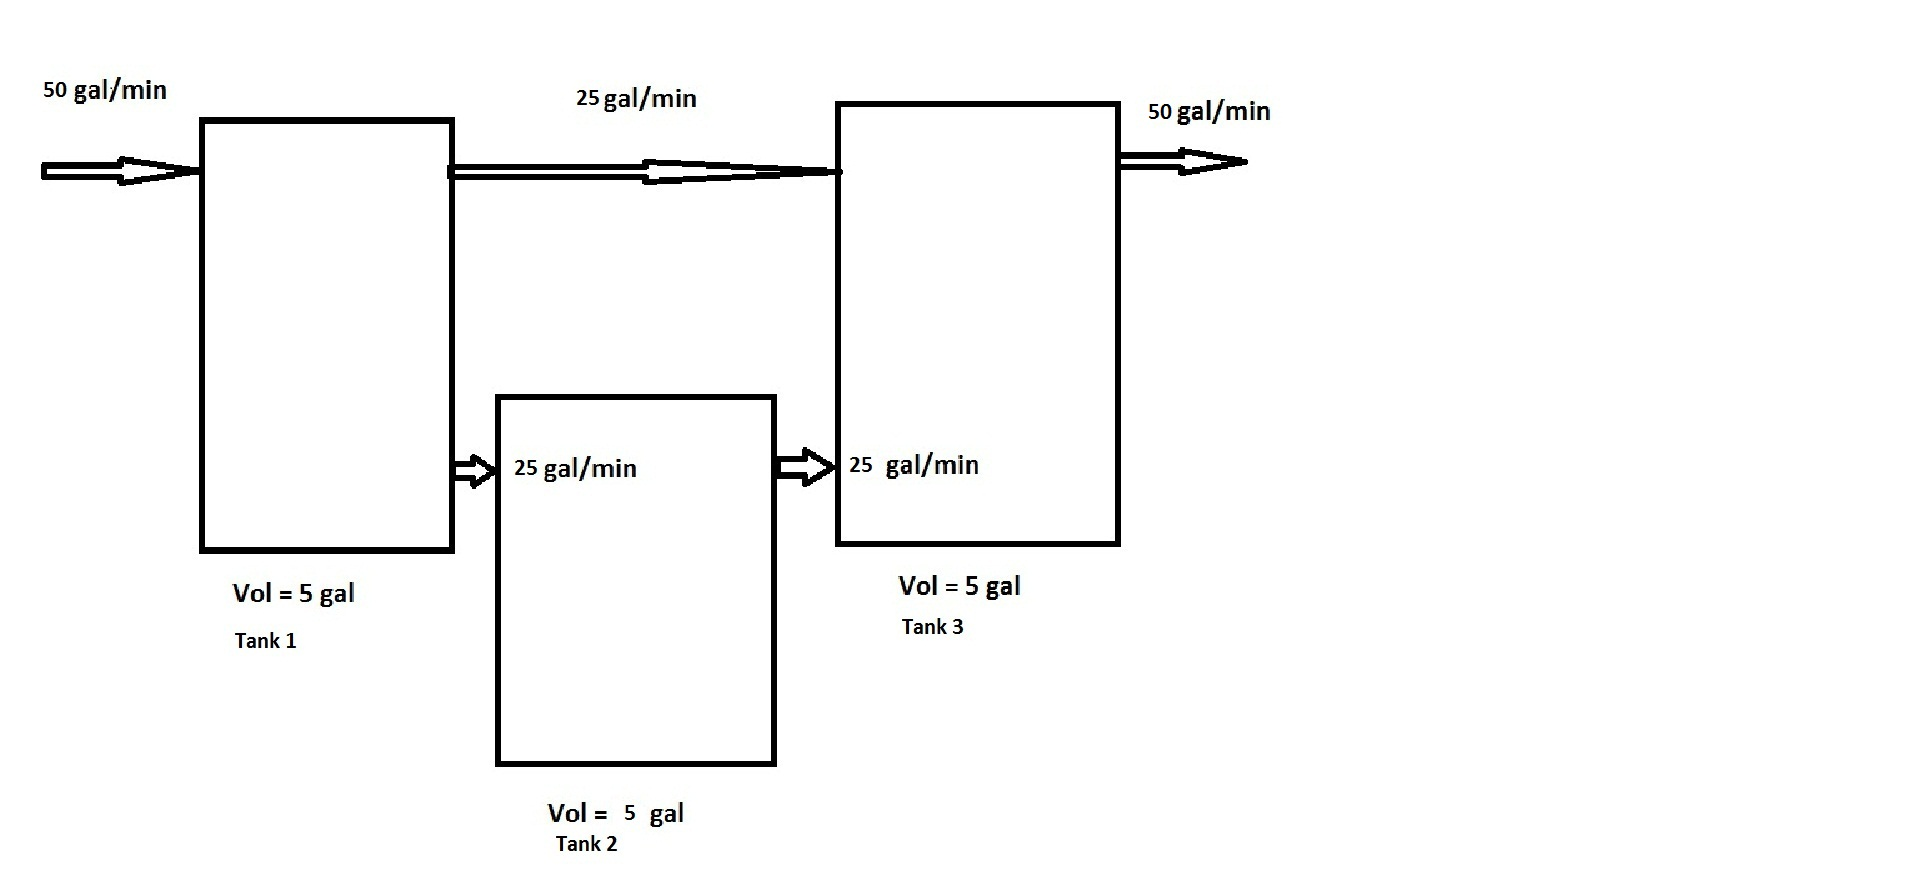
\includegraphics[scale=0.5]{SaltTank1.jpg}
%\caption{}
\end{center}
%\end{figure} 

\begin{enumerate}
\item[a.] Setup the IVP (a 3 by 3 first order linear system and initial data) that governs the amount of salt in
each tank after time $t$ minutes if initially $10$ lbs of salt are in tank 1, $2$ lbs are in tank 2, and tank 3 is 
empty of salt.

\bsni

\item[b.] Find the maximum amount of salt in tank 2 and when it occurs.

\end{enumerate}

\end{enumerate}

\end{document}